%----------- Necessary Style Preamble -----------%

\documentclass[mathserif, 10pt]{beamer} %

\usepackage[framesassubsections]{beamerprosper}
\usepackage{beamerthemesplit} % Activate for custom appearance
\usepackage[english]{babel}
\usepackage[latin1]{inputenc}
\usepackage{amsmath, hyperref, subfigure, multirow, rotating}
\usepackage{epstopdf}
\usepackage{verbatim}
\usepackage{listings}
\usepackage{color}
\usepackage{esint}
\usepackage{mathrsfs}
\usepackage{multicol}

%\usepackage{enumitem}

\usetheme{Frankfurt}
\usecolortheme{default}
\usecolortheme[rgb={0.1,0.4,0.0}]{structure} % CSU color style
%\usecolortheme[rgb={0.541,0.149,0.196}]{structure} % BME color style

\setbeamersize{text margin left=0.5cm}
\setbeamersize{text margin right=0.5cm}

\setbeamercovered{transparent}

\usepackage{remreset}
\makeatletter
\@removefromreset{subsection}{section}
\makeatother
\setcounter{subsection}{1}

\makeatletter
\newcommand\xleftrightarrow[2][]{\ext@arrow 0099{\longleftrightarrowfill@}{#1}{#2}}
\def\longleftrightarrowfill@{\arrowfill@\leftarrow\relbar\rightarrow}
\makeatother


\newcommand\Wider[2][3em]{%
\makebox[\linewidth][c]{%
  \begin{minipage}{\dimexpr\textwidth+#1\relax}
  \raggedright#2
  \end{minipage}%
  }%
}

%----------- Math Definitions -----------%

\definecolor{Blue}{rgb}{0,0,1}
\def\ci{\perp\!\!\!\perp}
\def\a{\mathbf{a}}
\def\d{\mathbf{d}}
\def\e{\mathbf{e}}
\def\f{\mathbf{f}}
\def\g{\mathbf{g}}
\def\b{\mathbf{b}}
\def\q{\mathbf{q}}
\def\v{\mathbf{v}}
\def\x{\mathbf{x}}
\def\y{\mathbf{y}}
\def\u{\mathbf{u}}
%\def\z{\mathbf{\mathfrak{z}}}
\def\z{\mathbf{z}}
\def\D{\mathbf{D}}
\def\S{\mathbf{S}}
\def\X{\mathbf{X}}
\def\Z{\mathbf{Z}}
\def\1{\raisebox{.5pt}{\textcircled{\raisebox{-.9pt} {1}}}}
\def\2{\raisebox{.5pt}{\textcircled{\raisebox{-.9pt} {2}}}}
\def\3{\raisebox{.5pt}{\textcircled{\raisebox{-.9pt} {3}}}}
\def\4{\raisebox{.5pt}{\textcircled{\raisebox{-.9pt} {4}}}}
\def\5{\raisebox{.5pt}{\textcircled{\raisebox{-.9pt} {5}}}}
\def\6{\raisebox{.5pt}{\textcircled{\raisebox{-.9pt} {6}}}}
\def\balph{\boldsymbol\alpha}
\def\bmu{\boldsymbol\mu}
\def\btheta{\boldsymbol\theta}
\def\bomega{\boldsymbol\omega}
\def\bDelta{\boldsymbol\Delta}

%----------- Title Page Parameters -----------%
\title[Digital Control \& Digital Filters]{Digital Controls \& Digital Filters \\ Lectures 23 \& 24}
\author[M.R. Azimi]{M.R. Azimi, Professor}
\institute[CSU-ECE]{Department of Electrical and Computer Engineering \\ Colorado State University}
\date{Spring 2017}

\logo{
\includegraphics[height=0.5cm]{csu-logo.png}}

\newcommand{\unt}[1]{ \mathrm{\ #1}}

\begin{document}

%----------- slide --------------------------------------------------%

\frame{\titlepage}




\section{Non-Recursive Digital Filter Design}
%----------- slide --------------------------------------------------%
\frame
{
%\vspace{-.2in}
\small
%\renewcommand{\theenumi}{\alph{enumi}}
\frametitle{Approximation Methods: FIR Digital Filters}

FIR filter are described by convolution summation:\\
$y(n) = \sum\limits_{k=0}^{N-1} h(k) x(n-k)$~~~~~
$x(n)$:  Input signal~~~
$y(n)$:  Output signal~\\
$h(n)$:  Impulse response (filter coefficients) \hspace{0.2in} $N$:  Filter order \\

\textcolor{red}{Advantages:}\\
\begin{enumerate}
	\item Inherently stable.
	\item Linear phase characteristic especially useful in applications where frequency dispersion due to non-linear phase is harmful e.g. speech and audio processing.
	\item Quantization effects can be made small.
	\item Implementation using parallel/pipeline processors because of inherent concurrency.
\end{enumerate}

\textcolor{red}{Disadvantages:}\\
\begin{enumerate}
	\item For a sharp cut-off performance a large order filter is required $\implies$ large computation time for implementation.
	\item In some cases "fractional delay" may be needed which can not be realized \\by physical devices.
\end{enumerate}

}


%----------- slide --------------------------------------------------%
\frame
{
\vspace{-.4in}
\small
%\renewcommand{\theenumi}{\alph{enumi}}
\frametitle{Frequency Response of FIR Filters}

The transfer function of a causal FIR filter is:\\ \vspace{.1in}
$H(z) = \sum\limits_{n=0}^{N-1} h(n) z^{-n}$\\
Let $z = e^{j\Omega}$ (i.e. unit circle)\\
$H(e^{j\Omega}) = \sum\limits_{n=0}^{N-1} h(n) e^{-j\Omega n} = DTFT\{h(n)\}$\\
Sampling the frequency scale $\Omega = \frac{2\pi k}{N}$ yields \\the $N$ elements of the DFT of $h(n)$ as:\\ \vspace{.1in}
$H(k) = \sum\limits_{n=0}^{N-1} h(n) e^{-\frac{2\pi j k n}{N}} = DFT \{h(n)\}, ~~k\in [0,N-1]$\\
and\\
$h(n) = IDFT\{H(k)\} = \frac{1}{N}\sum\limits_{k=0}^{N-1} H(k) e^{\frac{2 \pi j kn}{N}},~~n \in[0,N-1]$\\

Now, consider the following cases. \vspace{.1in}

\vspace{-2.4in}
\hspace{2.9in}
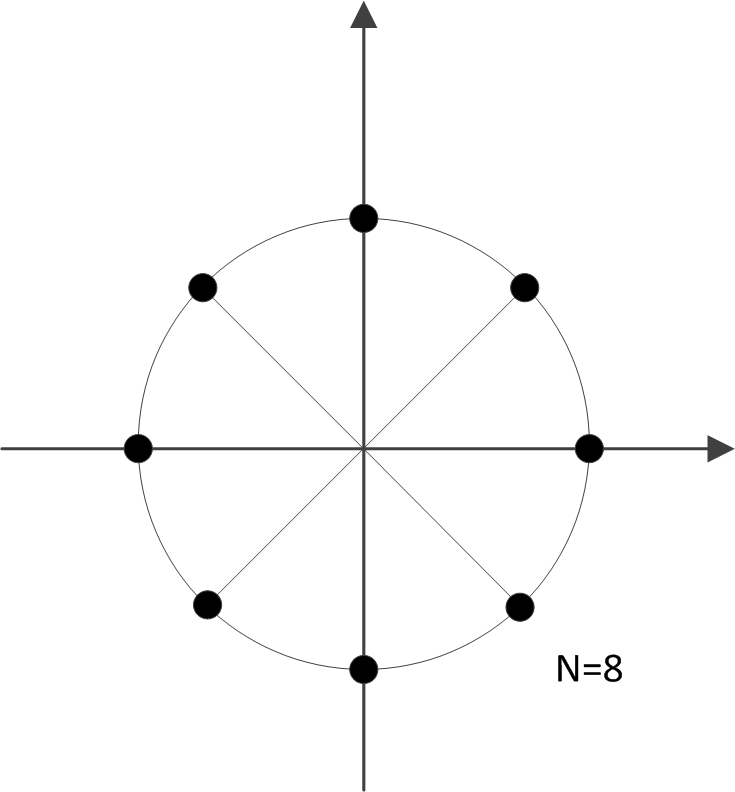
\includegraphics[width=.275\linewidth]{./Figures/sample.png}




}

%----------- slide --------------------------------------------------%
\frame
{

\small
%\renewcommand{\theenumi}{\alph{enumi}}
\frametitle{Frequency Response of FIR Filters-Cont.}
\textcolor{red}{Case 1:} Symmetric: $h(n) = h(N-1-n)$ and $N$ odd \\ \vspace{.1in}
$H(e^{j\Omega}) = e^{-j\Omega \frac{(N-1)}{2}}\sum\limits_{n=0}^{\frac{(N-1)}{2}} \alpha(n) \cos{\Omega n}$\\
where\\
$\alpha(n) \triangleq 2h\left[ \frac{(N-1)}{2}-n\right],~n\in[1,\frac{N-1}{2}]$\\
$\alpha(0) \triangleq h\left(\frac{(n-1)}{2}\right)$\\
$\phi(\Omega) = -\Omega\frac{(N-1)}{2}:$  linear\\ \vspace{.1in}
Group delay $\tau_g = -\frac{d\phi(\Omega)}{d\Omega} = \frac{N-1}{2}$:  Integer\\ \vspace{.2in}

\textcolor{red}{Case 2:} Symmetric: $h(n) = h(N-1-n)$ and $N$ Even \\ \vspace{.1in}
$H(e^{j\Omega}) = e^{-j\Omega\frac{(N-1)}{2}}\sum\limits_{n=1}^{N/2} \beta(n) \cos{[\Omega(n-1/2)]}$\\
where,\\
$\beta(n) \triangleq 2h(\frac{N}{2}-n), ~~n\in[1,N/2]$\\ \vspace{.07in}
Note that at $\Omega = \pi, H(e^{j\Omega}) = 0$ i.e HPF can not be approximated.


}


%----------- slide --------------------------------------------------%
\frame
{

\normalsize
%\renewcommand{\theenumi}{\alph{enumi}}
\frametitle{Frequency Response of FIR Filters-Cont.}

\textcolor{red}{Case 3:} Anti-Symmetric:  $h(n) = -h(N-1-n)$, $h(\frac{N-1}{2})=0$, and  $N$ odd \\ \vspace{.1in}
$H(e^{j\Omega}) = e^{-j\Omega \frac{(N-1)}{2}}e^{j\pi/2}\sum\limits_{n=1}^{\frac{(N-1)}{2}} \gamma(n) \sin{\Omega n}$\\
where\\
$\gamma(n) \triangleq 2h\left[ \frac{(N-1)}{2}-n\right],~n\in[1,\frac{N-1}{2}]$\\ \vspace{.2in}
%$\gamma(0) \triangleq h\left(\frac{(n-1)}{2}\right)$\\ \vspace{.2in}

\textcolor{red}{Case 4:} Anti-Symmetric:  $h(n) = -h(N-1-n)$ and $N$ even \\ \vspace{.1in}
$H(e^{j\Omega}) = e^{-j\Omega\frac{(N-1)}{2}}e^{j\pi/2}\sum\limits_{n=1}^{N/2} \delta(n) \sin{[\Omega(n-1/2)]}$\\
where,\\
$\delta(n) \triangleq 2h(\frac{N}{2}-n), ~~n\in[1,N/2]$ \\ \vspace{.1in}

In the anti-symmetric case at $\Omega = 0, H(e^{j\Omega}) = 0$.  i.e. suitable for approximating such filters as differentiators and Hilbert transforms

}

%----------- slide --------------------------------------------------%
\frame
{

\small
%\renewcommand{\theenumi}{\alph{enumi}}
\frametitle{Frequency Sampling Method}
\textcolor{red}{Design Methods}
\begin{enumerate}
	\item Windowing
	\item Frequency sampling method
	\item Computer aided design methods (CAD)
\end{enumerate}
\textcolor{blue}{Frequency Sampling Method}\\
\textbf{Idea:} Given the frequency response of the desired filter, $H_{Des}(e^{j\Omega})$, sample it to obtain $H(k)$ and then take IDFT of $\{H(k)\}$ to get $\{h(n)\}$. \\ \vspace{.15in}
Let the transfer function of the FIR filter be :\\
$H(z) = \sum\limits_{n=0}^{N-1} h(n) z^{-n}$\\
we know that \\
$H(k) = H(z)|_{z = \frac{j2\pi k}{N}} = \sum\limits_{n=0}^{N-1} h(n) e^{\frac{-j2 \pi kn}{N}}, ~~~k \in [0,N-1]$\\ \vspace{.05in}
Additionally: $h(n) = IDFT \{H(k)\} = \frac{1}{N} \sum\limits_{k=0}^{N-1} H(k) e^{\frac{j2\pi kn}{N}}, ~~~n\in[0,N-1]$\\

Then, \\

$H(z) = \sum\limits_{n=0}^{N-1} \left[ \frac{1}{N}\sum\limits_{k=0}^{N-1} H(k) e^{\frac{j2\pi kn}{N}}\right]z^{-n} = \sum\limits_{k=0}^{N-1} \frac{H(k)}{N}\sum\limits_{n=0}^{N-1}(e^{\frac{j2\pi k}{N}}z^{-1})^n$


}

%----------- slide --------------------------------------------------%
\frame
{

\small
%\renewcommand{\theenumi}{\alph{enumi}}
\frametitle{Frequency Sampling Method-Cont. }
Now using $\sum\limits_{n=0}^{N-1} a^n = \frac{1-a^N}{1-a}$, we get ,\\

$\sum\limits_{k=0}^{N-1} \frac{H(k)}{N}\frac{(1-e^{j2 \pi k}z^{-N})}{(1-e^\frac{j2 \pi k}{N}z^{-1})} = \underbrace{\frac{(1-z^{-N})}{N}}_{H_1(z)} \underbrace{\sum\limits_{k=0}^{N-1}\frac{H(k)}{(1-e^\frac{j2 \pi k}{N}z^{-1})}}_{H_2(z)}$\\
which can be realized by cascade of a simple FIR (Comb) filter with an IIR system. \\ \vspace{.1in}

\hspace{1in}
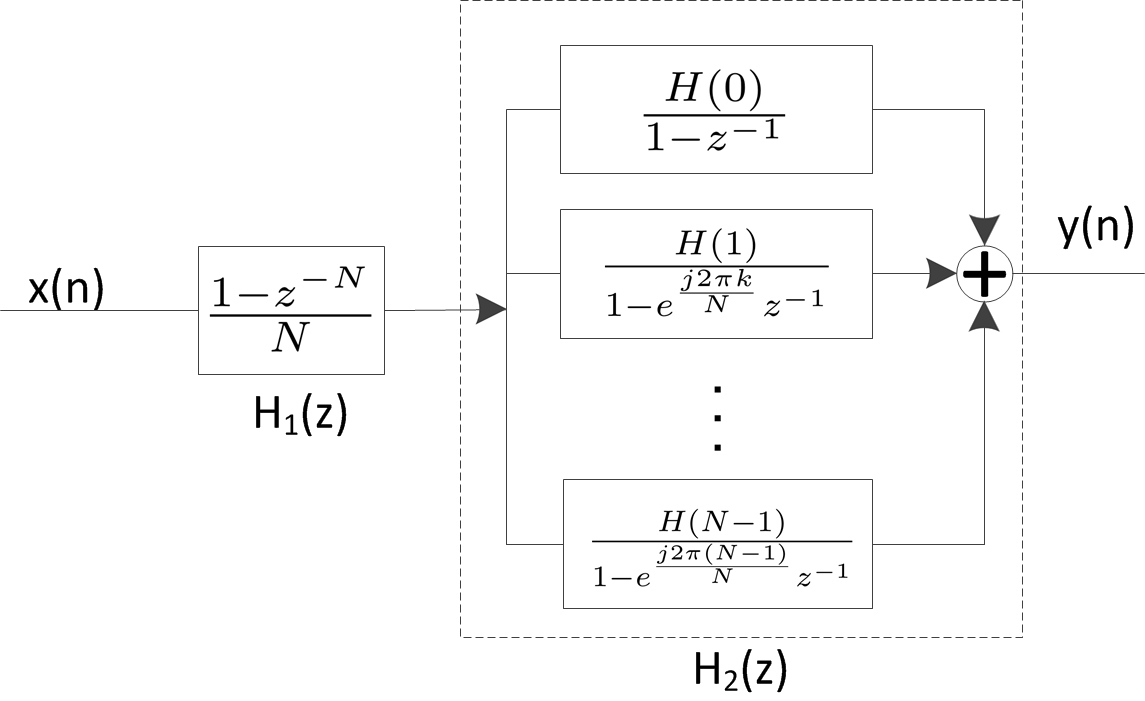
\includegraphics[width=.55\linewidth]{./Figures/cascade.png}

}

%----------- slide --------------------------------------------------%
\frame
{

\normalsize
%\renewcommand{\theenumi}{\alph{enumi}}
\frametitle{Frequency Sampling Method}
The term $(1-z^{-N})$ represents an FIR filter with frequency response $H_1(e^{j\Omega}) = 1-e^{-j\Omega N} = e^{-j\Omega \frac{N}{2}}\left[e^{j\Omega\frac{N}{2}}-e^{-j\Omega\frac{N}{2}}\right] = e^{-j\Omega\frac{N}{2}}2j \sin\frac{\Omega N}{2}$ \\

The plot of $|H_1(e^{j\Omega})|$ as a function of $\Omega$  is shown below. \vspace{.1in}

\hspace{1in}
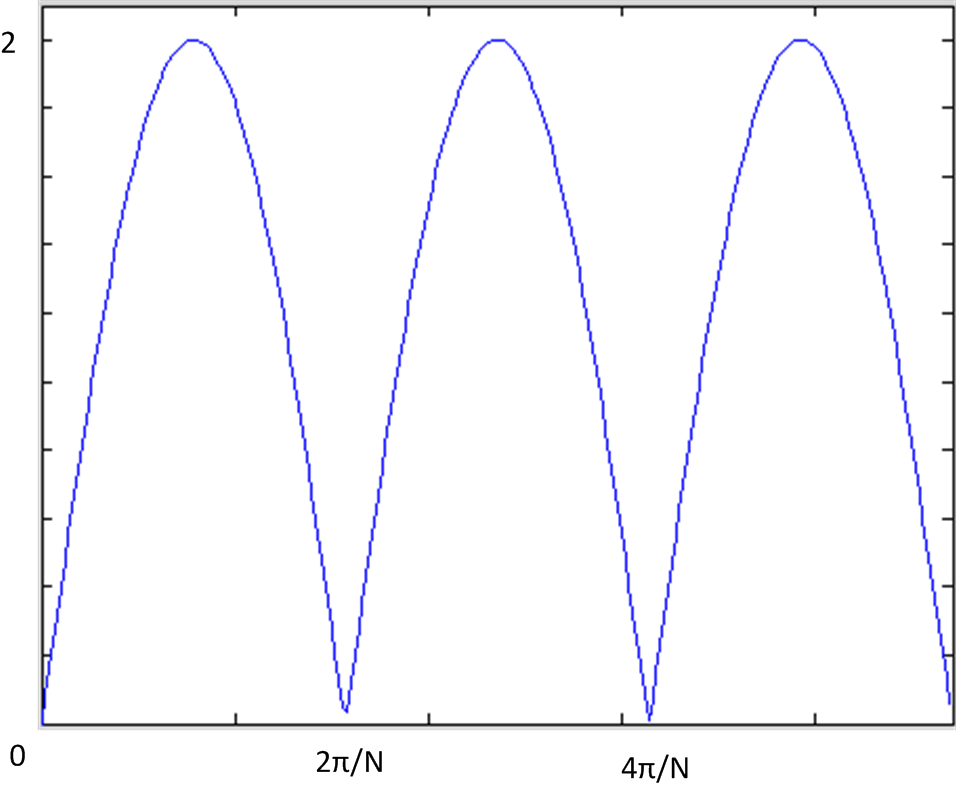
\includegraphics[width=.5\linewidth,height=1in]{./Figures/comb.png} \vspace{.1in}

The IIR part, $H_2(z)$, consists of parallel combination of $N$ complex coefficient 1st order systems with poles at $z_k = e^{\frac{j2\pi k}{N}}$ on the unit circle.  Of course these poles will be cancelled with the zeros of $H_1(z)$ which also occur at $z_k = e^{\frac{j2\pi k}{N}}$ since $1-z^{-N} =0  \implies z = (1)^{1/N} \implies z_k = e^\frac{j2\pi k}{N}, ~~k\in[0,N-1]$\\ \vspace{.1in}

}

%----------- slide --------------------------------------------------%
\frame
{

\small
%\renewcommand{\theenumi}{\alph{enumi}}
\frametitle{Frequency Sampling Method}

In order to have $H(z)$ with real coefficients (physical realization) we require that $H(k)=|H(k)| e^{j\theta(k)}$ satisfy:\\ \vspace{.15in}
$|H(k)| = |H(N-k)|$ \\
and \\
$\theta(k) = -\theta(N-k), ~~k\in[0,N-1]$\\ \vspace{.1in}
Now each pair of $ H(k)$ and $H(N-k),~~k\in[0,\frac{N}{2}]$ gives a 2nd order system with real coefficients.  i.e:
$H_k(z) = \frac{H(k)}{1-e^\frac{j2\pi k}{N}z^{-1}}+\frac{H(N-k)}{1-e^\frac{j2\pi (N-k)}{N}z^{-1}} = \frac{2|H(k)|[\cos{\theta(k)} -z^{-1} \cos{(\theta(k)-\frac{2\pi k}{N})}]}{1-2 \cos\frac{2\pi k}{N}z^{-1}+z^{-2}}$  \\ \vspace{.1in}
Note that for $N$ odd there is no frequency sample for $k=N/2$ thus the corresponding term does not exist.

}

%----------- slide --------------------------------------------------%
\frame
{

\small
%\renewcommand{\theenumi}{\alph{enumi}}
\frametitle{Frequency Sampling Method: Design Procedure}

Given desired frequency response $H_{Des}(e^{j\Omega})$ sample it to yield:\\ \vspace{.1in}
$H(k) = H_{Des}(e^{j\Omega})|_{\Omega = \frac{2\pi k}{N}},~~k\in[0,N-1]$\\ \vspace{.1in}
Impose the following conditions on the magnitude $|H(k)|$ and phase $\theta(k)$:\\ \vspace{.1in}
\begin{enumerate}
	\item \textit{\textbf{For linear phase:}}  $\theta(k) = -\frac{(N-1)k\pi}{N},~~k\in[0,N-1]$
	\item \textit{\textbf{For real coefficients:}}
	$|H(k)| = |H(N-k)|$ and $\theta(k) = -\theta(N-k)$ \\ \vspace{.1in}
Note for $N$ even set $H(\frac{N}{2})=0$.
\end{enumerate}

\textcolor{red}{Example:} Design an $N=11$ order low-pass FIR filter whose cut-off frequency $f_c=2f_s/11$,
where $f_s$ is the sampling frequency. Plot the magnitude response of the designed filter. \\ \vspace{.07in}
We start with ideal filter for $H_{Des}(e^{j\Omega})$ and sample it with spacing between samples= $\frac{\Omega_s}{2\pi N}=\frac{f_s}{N}$. See below figure. \\
\begin{center}
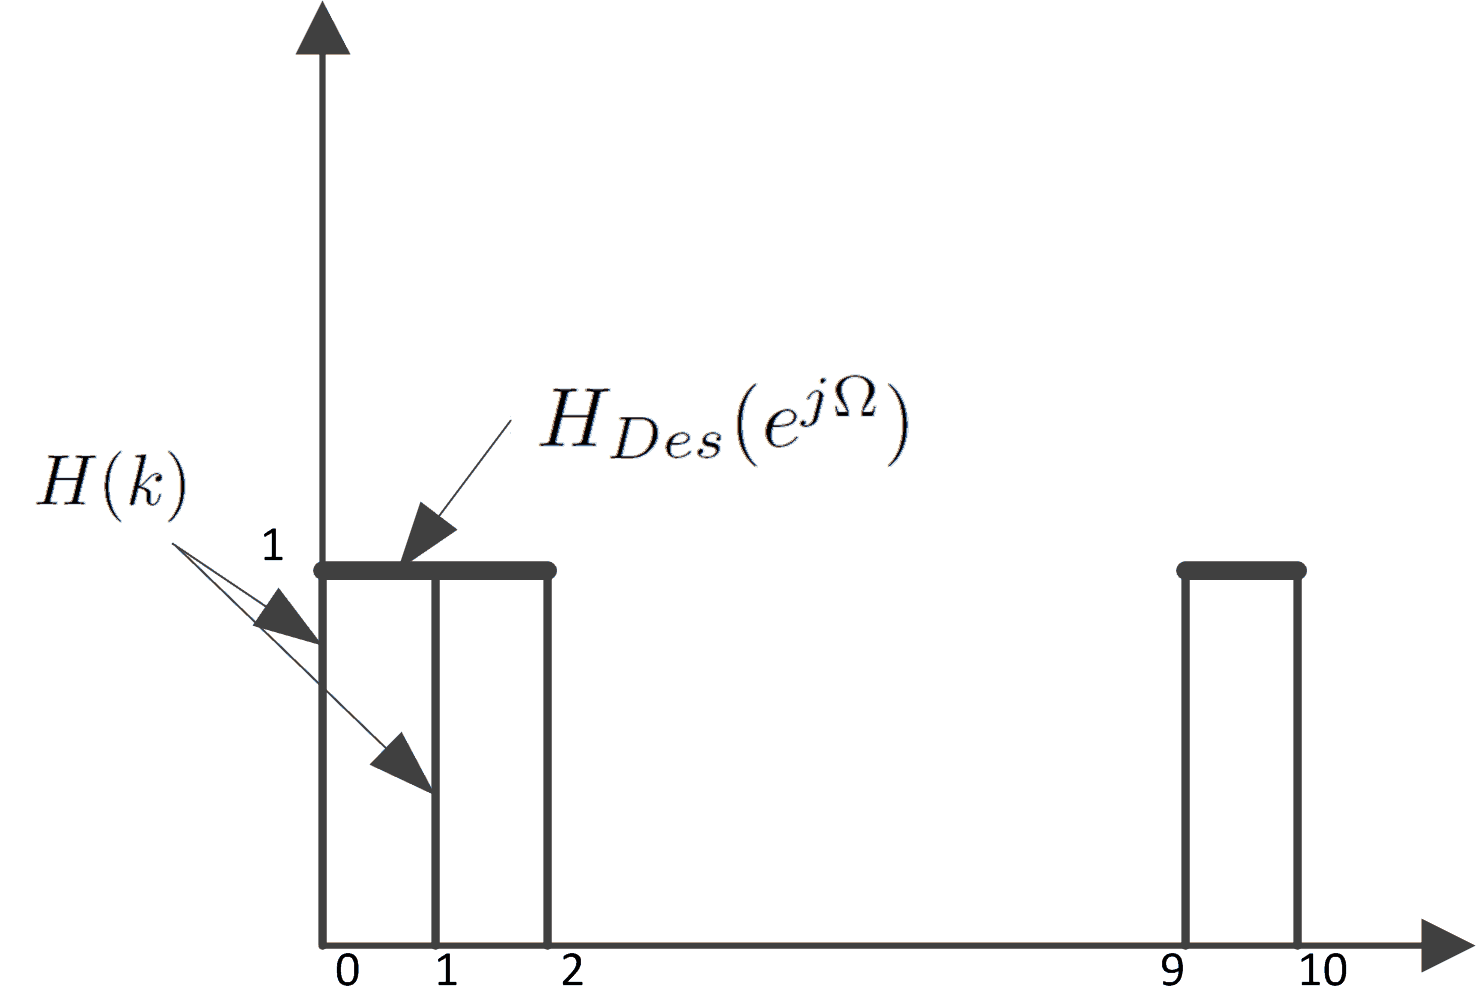
\includegraphics[width=.22\linewidth]{./Figures/Frequency-samplingex.png}
\end{center}


}

%----------- slide --------------------------------------------------%
\frame
{

\small
%\renewcommand{\theenumi}{\alph{enumi}}
\frametitle{Frequency Sampling Method: Design Procedure}
We then impose the above conditions i.e. \\ \vspace{.1in}

$|H(k)| = |H(N-k)|$ and \\ \vspace{.07in}

$\theta(k) = -\frac{(N-1)k\pi}{N}=\frac{10k\pi}{11},~~k\in[0,10]$ \\ \vspace{.07in}

These combined yield, \\ \vspace{.1in}

$H(k)=\left\{\begin{array}{ll} e^{-j\frac{10k\pi}{11}} ~~~ k = 0,1,2 ~~~~~\text{and} ~~~~ k=9,10
\\ 0 ~~~~~~~~~~~k\in[3,8] \end{array} \right$ \\ \vspace{.1in}

Then take size $N=11$ IDFT of $H(k)$ i.e. $h(n)=IDFT\{H(k)\}_{11}$ which gives\\ \vspace{.07in}

$h(0)=0.06942, ~~h(1)=-0.05403, ~~h(2)=-0.10945, ~~h(3)=0.04733,$
$h(4)=0.31938, ~~h(5)=0.45455, ~~h(6)=0.31938, ~~h(7)=0.04733,$
$h(8)=-0.10945, ~~h(9)=-0.05403, ~~h(10)=0.06942$ \\ \vspace{.1in}

Note that these are symmetric due to the linear phase condition imposed. Magnitude response of the designed filter is shown (thick line)
which exhibits a rather large ripple in both passband and stopband. \\

To reduce the ripple effect, one can add a sample in the transition (wider transition region) region, i.e.\\ \vspace{.1in}
}

%----------- slide --------------------------------------------------%
\frame
{

\small
%\renewcommand{\theenumi}{\alph{enumi}}
\frametitle{Frequency Sampling Method: Design Procedure}
\begin{center}
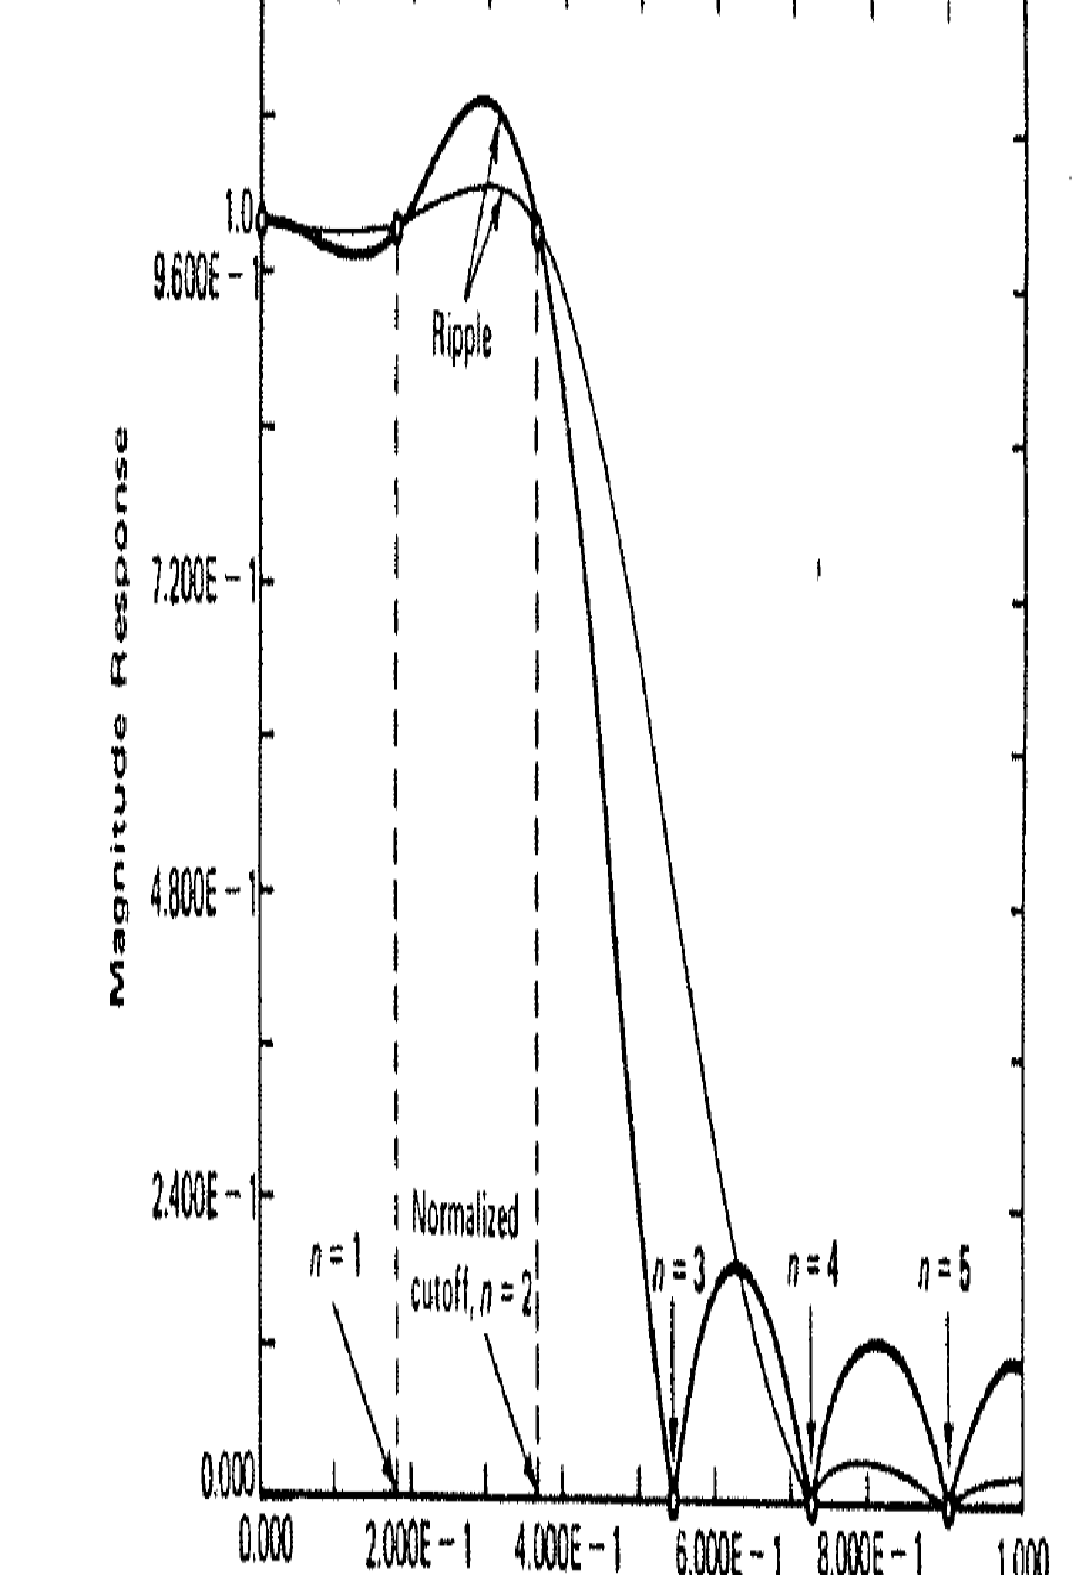
\includegraphics[width=.35\linewidth,height=.8in]{./Figures/mag-response.pdf}
\end{center}


$H(k)=\left\{\begin{array}{ll} e^{-j\frac{10k\pi}{11}} ~~~ k = 0,1,2 ~~~~~\text{and} ~~~~ k=9,10 \\
0.5e^{-j\frac{10k\pi}{11}} ~~~ k = 3 ~~~~~\text{and} ~~~~ k=8
\\ 0 ~~~~~~~~~~~k\in[4,7] \end{array} \right$ \\ \vspace{.1in}

The resulting filter coefficients are: \\

$h(0)=0.00987, ~~h(1)=0.02244, ~~h(2)=-0.07168, ~~h(3)=-0.03989,$
$h(4)=0.30643, ~~h(5)=0.54545, ~~h(6)=0.30643, ~~h(7)=-0.03989,$
$h(8)=-0.07168, ~~h(9)=0.02244, ~~h(10)=0.00987$ \\ \vspace{.1in}

The magnitude response is shown (thin line) which shows much less
ripple effects at a cost of wider transition region (must increase the order). Note that one can try to optimize the choice of the amplitude
of the introduced sample.



}

\section{Digital Controller Design}

%----------- slide --------------------------------------------------%
\frame
{

\small
%\renewcommand{\theenumi}{\alph{enumi}}
\frametitle{Design of Digital Controller-Classical method}
\textbf{Goal: } Design compensators to achieve certain desired characteristics e.g., steady-state accuracy, transient response, relative stability, sensitivity, etc.\\
\begin{enumerate}
	\item \textit{Steady-State Accuracy:} \\
	Desired $e_{ss} \approx 0 \implies $poles at $z=1 \implies$ more lags $\implies$ less stable
	\item \textit{Transient Response:}\\
	Desired:  Reduce $t_r \implies$ increase BW $\implies$ less noise immunity
	\item \textit{Relative Stability:}\\
	Desired:  Small $M_p \implies$ increase in $t_r$ $\implies$ slower response
	\item \textit{Sensitivity:} Variation of system parameters wrt change in temperature, humidity, aging, altitude, etc.\\
	Measured by $S_{\alpha}^{T}=\frac{\partial T}{\partial \alpha}.\frac{a}{T}$ where $T(z)=\frac{G(z)}{1+G(z)}$ and $\alpha$ is a system parameter, e.g.,  \\ \vspace{.1in}

$S_{G}^{T}= \frac{1}{1+G(z)}$ or in frequency domain $S_{G}^{T}= \frac{1}{1+G(e^{j\Omega})}$ which implies, \\ \vspace{.1in}
Reduce sensitivity $S_{G}^{T} \implies$ Increase open loop gain $G(e^{j\Omega}) \implies $ Instability problems.

\end{enumerate}


}

%----------- slide --------------------------------------------------%
\frame
{

\small
%\renewcommand{\theenumi}{\alph{enumi}}
\frametitle{Digital PID Controller}

Recall from ECE 411, for PID controller: \\  \vspace{.05in}
$G_c(s) = K_P+K_I/s +K_Ds$\\  \vspace{.05in}
where $K_P$: proportional gain, $K_I$ integrator gain, and $K_D$ derivative gain. \\ \vspace{.05in}

Though bilinear $z$-mapping can be used for the integrator:\\ \vspace{.05in}
$1/s \to \frac{T}{2}\frac{(z+1)}{z-1)}$\\ \vspace{.05in}
it \underline{cannot} be used for the derivative part. But we can use backward difference method: \\ \vspace{.05in}
$y(t) = \frac{dx(t)}{dt} \approx \frac{x(t)-x(t-\Delta T)}{\Delta T}$, $\Delta T=1, t = nT$\\ \vspace{.05in}
$y(n) = \frac{x(n)-x(n-1)}{T} \implies Y(z) = \frac{(X(z)-z^{-1}X(z))}{T} \implies \frac{Y(z)}{X(z)} = \frac{(z-1)}{zT}$\\ \vspace{.05in}
Thus, the mapping is $s \to \frac{(z-1)}{Tz}$ which yields digital PID transfer function: \\ \vspace{.05in}
$G_c(z) = K_P +K_I \frac{T}{2} \frac{(z+1)}{(z-1)}+ K_D \frac{(z-1)}{Tz} =\frac{a_0z^2+a_1z+a_2}{z(z-1)}$:  Second order IIR filter \\ \vspace{.05in}
where  $a_0 = K_P +K_IT/2+K_D/T$,  $a_1 = -K_P+K_IT/2-2K_D/T$, $a_2 = K_D/T$, $b_1=-1$, and $b_2=0$ \\ \vspace{.05in}

Design of PID controllers involves finding $K_P$, $K_I$, and $K_D$ to meet the desired performance criteria.
}

%----------- slide --------------------------------------------------%
\frame
{

\small
%\renewcommand{\theenumi}{\alph{enumi}}
\frametitle{Digital PID Controller-Cont.}
\textcolor{red}{Example:} Given plant transfer function, $G_p(s) = \frac{10}{(s+1)(s+2)}$,  design a PID controller $D(z)$ to meet desired specs. \\ \vspace{.15in} \\
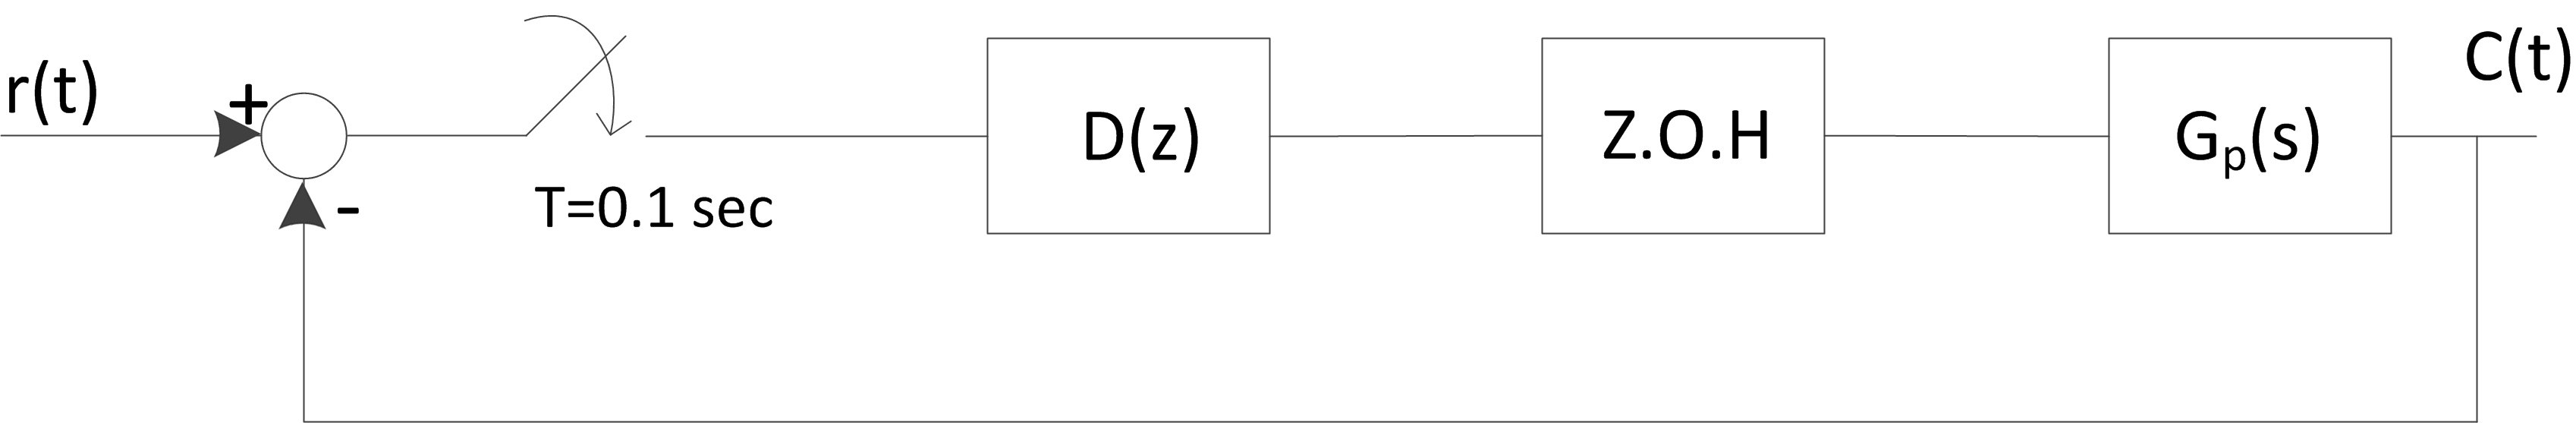
\includegraphics[width=.75\linewidth]{./Figures/example_diag.png} \\
Loop transfer function is, \\ \vspace{.08in}
$G(z) = D(z)(1-z^{-1})\Z\left[ \frac{10}{s(s+1)(s+2)} \right] = D(z)\frac{0.0453(z+0.904)}{(z-0.905)(z-0.819)}$\\ \vspace{.08in}

First consider the uncompensated case, $D(z) = 1$, then closed loop transfer function is: \\ \vspace{.1in}

$T(z) = \frac{C(z)}{R(z)}=\frac{G(z)}{1+G(z)} = \frac{0.0453(z+0.904)}{z^2-1.679-0.782}$\\ \vspace{.07in}
The CE is, \\
$\rho(z) = z^2-1.68z+0.78 = 0 \implies z_{1,2} = 0.84 \pm j0.28$ \\ \vspace{.07in}
Hence $|z_{1,2}| \approx 0.885 < 1\implies$ i.e. stable \\ \vspace{.07in}

However, since the loop transfer function doesn't have any pole at $z=1$, steady-state error is not zero. \\


}

%----------- slide --------------------------------------------------%
\frame
{

\small
%\renewcommand{\theenumi}{\alph{enumi}}
\frametitle{Digital PID Controller-Cont.}
$c_{ss} = \lim\limits_{z\to1}(1-z^{-1})C(z)= \lim\limits_{z\to1} \frac{0.0453(z+0.904)}{z^2-1.679-0.782}= 0.84$ \\ \vspace{.07in}
Thus, $e_{ss}=1-0.84=0.16$.  The step response is shown below which reveals this fact. \\ \vspace{.1in}
\hspace{1in}
\includegraphics[width=.4\linewidth]{./Figures/example_graph.png} \\

For $e_{ss}=0$ we then use an integral controller, \\ \vspace{.07in}
$D(z) = K_P+K_I\frac{T}{2}\frac{(z+1)}{(z-1)} = \frac{(K_IT+2K_P)z+(K_IT-2K_P)}{(z-1)}$\\ \vspace{.07in}
Then, the loop transfer function becomes, \\
$G(z) = D(z)\frac{0.0453(z+0.904)}{(z-0.905)(z-0.819)(z-1)} = \frac{(2K_P+K_IT)(z+\frac{K_IT-2K_P}{K_IT+2K_p})(z+0.094)}{(z-1)(z-0.905)(z-0.819)}$\\



}

%----------- slide --------------------------------------------------%
\frame
{

\small
%\renewcommand{\theenumi}{\alph{enumi}}
\frametitle{Digital PID Controller-Cont.}

Clearly, $e_{ss} = 0$ because of pole at $z=1$. To simplify the design, we choose $K_I$ and $K_P$ to cancel pole at $z=0.905$ (near unit circle)\\ \vspace{.07in}
$\frac{K_I-2K_P}{K_IT+2K_P} = -0.905 \implies \frac{K_P}{K_I} = 1.0026$\\ \vspace{.1in}
Now, choose $K_P = 1 \implies K_I = 0.997$\\ \vspace{.07in}
$D(z) = \frac{1.05(z-0.905)}{(z-1)}$\\ \vspace{.07in}
The loop transfer function with PI controller:\\ \vspace{.07in}
$G(z) =\frac{0.0453(z+0.904)}{(z-1)(z-0.819)}$ \\ \vspace{.07in}

Step response for three different values \\
 of $K_P$ and hence $K_I$ are shown. As can \\
 be seen the response either has a high \\
 Max overshoot or long rise  time. \\ \vspace{.07in}


\vspace{-.65in}
\hspace{2.25in}
\includegraphics[width=.4\linewidth]{./Figures/PI_graphs.png}

}

%----------- slide --------------------------------------------------%
\frame
{

\small
%\renewcommand{\theenumi}{\alph{enumi}}
\frametitle{Digital PID Controller-Cont.}

We can achieve both goals while $e_{ss}=0$ using a PID controller,  \\ \vspace{.07in}

$D(z)= \frac{a_0z^2+a_1z+a_2}{z(z-1)}$ \\ \vspace{.1in}

The PID parameters $K_P,K_I,K_D$  must be determined to satisfy certain desired specs.
First, we choose to cancel both poles of uncompensated system with those of PID. Additionally,
we add another requirement that ramp error constant \\ \vspace{.07in}
 $K_v=5 \implies e_{ss}=1/K_v=1/5=0.2$. \\ \vspace{.07in}

$K_v=\frac{1}{T} \lim\limits_{z\to1}(1-z^{-1})G(z)=5K_I \implies K_I=1$ \\ \vspace{.07in}

$a_0z^2+a_1z+a_2 = (z-0.905)(z-0.819)$\\ \vspace{.07in}
$\left\{\begin{array}{l}
a_0 = K_P+K_I \frac{T}{2}+\frac{K_D}{T}\\
a_1= K_I \frac{T}{2} - K_P-\frac{2K_D}{T}\\
a_2 = \frac{K_D}{T}
\end{array} \implies
\begin{array}{l}
K_P = 1.45\\
K_D = 0.43 \\
K_I=1
\end{array} \right.$\\

The loop transfer function and closed-loop transfer function are, \\ \vspace{.07in}

$G(z) = \frac{0.263(z+0.904)}{z(z-1)}$\\ \vspace{.07in}
$T(z) = \frac{0.263(z+0.904)}{z^2-0.737z+0.238}$

}

%----------- slide --------------------------------------------------%
\frame
{

\small
%\renewcommand{\theenumi}{\alph{enumi}}
\frametitle{Digital PID Controller-Cont.}

For this system CE is, \\ \vspace{.07in}
$\rho(z) = z^2-0.737z+0.238 = 0 \implies z_{1,2} = 0.37 \pm j0.32$ \\ \vspace{.07in}
Hence $|z_{1,2}| \approx 0.48 < 1\implies$ i.e. much closer to the origin of the unit circle. \\ \vspace{.07in}

The step response is shown which has a max overshoot of 4\% while offering a good rise time. \\ \vspace{.07in}

\vspace{-.08in}
\hspace{1.6in}
\includegraphics[width=.35\linewidth]{./Figures/PID_graph.png}

}


\end{document}

